\section*{RESULTS}\label{results}

    \subsection*{Roll decay model tests}\label{roll-decay-model-tests}

\subsubsection*{Test at 0 knots}\label{test-at-0-knots}

Two roll decay model tests were conducted at zero speed referred to as
Run 1 and 2.
These tests where analyzed by fitting a cubic model
to the model test data. The two models were very similar in terms of
roll damping and stiffness (see Fig.\ref{fig:mdl}), suggesting
good repeatability in both the model tests and in the parameter
identification technique (PIT) used. It can be seen that the dampings,
from each individual oscillation obtained with the logarithmic decrement
method, are very scattered. This scatter does not seem to influence the
two models for the 0 speed case, which are very similiar.

    \subsubsection*{Test at 15.5 knots}\label{test-at-15.5-knots}

One roll decay model tests, referred to as Run 3, was conducted at a
ship speed corresponding to 15.5 knots full scale ship speed (see
Fig.\ref{fig:mdl}). The ship got a small yaw rate
 at the end of test, giving a small steady roll angle due to the
centrifugal force. Since this effect is not included in the matematical
model used, the steady roll angle was instead removed by removing the
linear trend in the roll angle signal.

    

    \begin{figure}[H]
        \begin{center}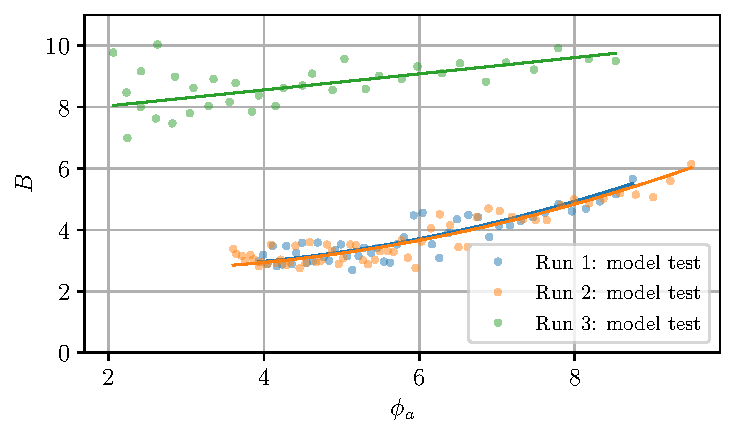
\includegraphics[width = 0.5\textwidth]{figures/mdl.pdf}\end{center}
        \vspace{-1cm}
        \caption{Model test roll damping}
        \label{fig:mdl}
    \end{figure}
    
    \subsection*{Damping by Ikeda's method}\label{damping-by-ikedas-method}

    The $C_r$ was calculated with regular Ikeda's method and the
alternative decision tree model for the KVLCC2 with section data
according to tab.\ref{tab:kvlcc2_section_table}. A comparison
between these two methods are shown in
Fig.\ref{fig:analytical_numerical}. It can be seen that the
regular implementation of Ikeda's method predicts much higher $C_r$
between station 8 and 14, where the bilge radius is also very small for
this ship.

    

    \begin{figure}[H]
        \begin{center}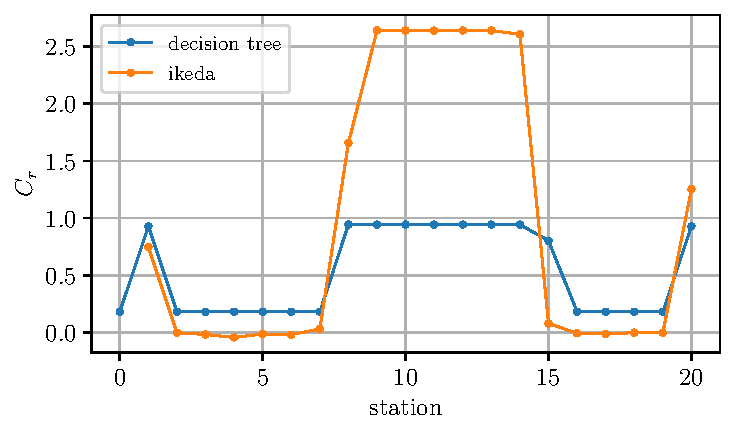
\includegraphics[width = 0.5\textwidth]{figures/kvlcc2_eddy.pdf}\end{center}
        \vspace{-1cm}
        \caption{KVLCC2 eddy damping coefficient along the hull}
        \label{fig:kvlcc2_eddy}
    \end{figure}
    
    When looking at predictions in Fig.\ref{fig:ikeda} for KVLCC2 at
0 speed made with regular Ikeda's method (left), it was found that the
eddy damping $B_E$ was too high compared to the model test results.
Even though the rest of the components would also be overpredicted, the
$B_E$ would still be too large. The eddy damping calculated with
$C_r$ predicted with the descision tree gave much better agreement and
is instead used in the hybrid method.

    

    \begin{figure}[H]
        \begin{center}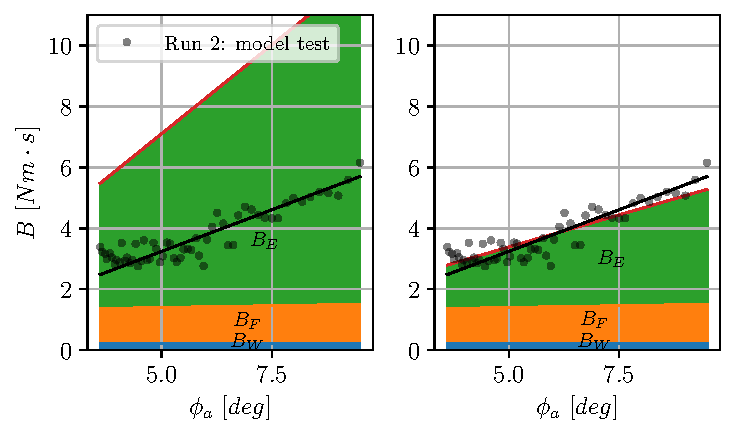
\includegraphics[width = 0.5\textwidth]{figures/ikeda.pdf}\end{center}
        \vspace{-1cm}
        \caption{Roll damping components calculated with the two implementations of Ikeda's method.}
        \label{fig:ikeda}
    \end{figure}
    
    \subsection*{Motions estimated by FNPF}\label{motions-estimated-by-fnpf}

Simulations of roll decay tests were conducted with FNPF without viscous
damping. Wave damping obtained from these tests are shown in
Fig.\ref{fig:fnpf}. This damping term does not seem to change
much with the roll amplitude. This means that the wave damping is
reasonably linear, which confirms Ikeda's original assumption used in
his derivation of the eddy damping \citep{7505983/4AFVVGNT}.

    

    \begin{figure}[H]
        \begin{center}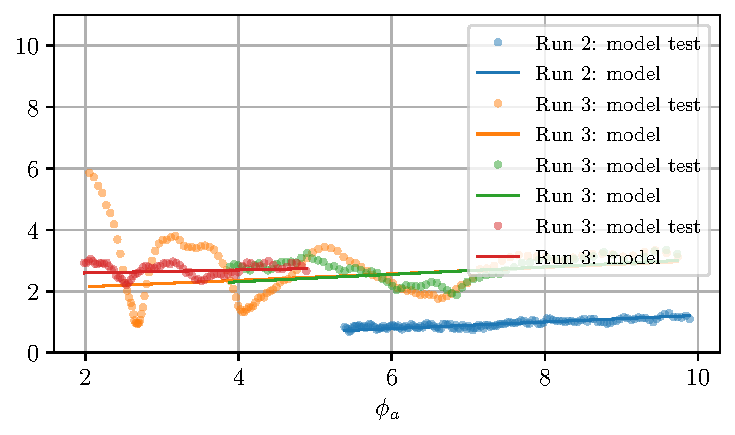
\includegraphics[width = 0.5\textwidth]{figures/fnpf.pdf}\end{center}
        \vspace{-1cm}
        \caption{Wave damping obtained from FNPF}
        \label{fig:fnpf}
    \end{figure}
    
    \subsection*{Roll motion prediction with hybrid
method}\label{roll-motion-prediction-with-hybrid-method}

    In Fig.\ref{fig:ikeda} the wave damping $B_W$ was calculated
using a linear strip theory. If this damping is instead replaced by the
wave damping from FNPF (as shown in Fig.\ref{fig:fnpf}) the
total damping is instead as shown in Fig.\ref{fig:hybrid_0}.

    

    \begin{figure}[H]
        \begin{center}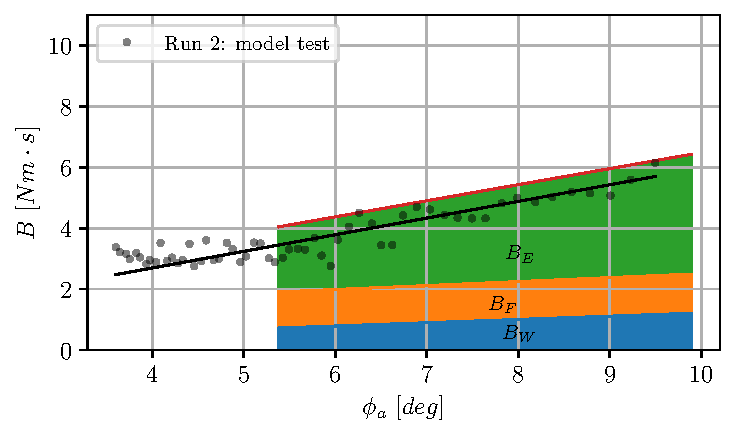
\includegraphics[width = 0.5\textwidth]{figures/hybrid_0.pdf}\end{center}
        \vspace{-1cm}
        \caption{Roll damping from hybrid method (0 kn)}
        \label{fig:hybrid_0}
    \end{figure}
    
    Results from the roll decay model test and corresponding simulations
with hybrid method and FNPF method is shown in
Fig.\ref{fig:analytical_numerical}. It is very clear that the
injection of semi empirical viscous damping in the hybrid method has
given a significant improvement compared to the invicid FNPF.

    

    \begin{figure}[H]
        \begin{center}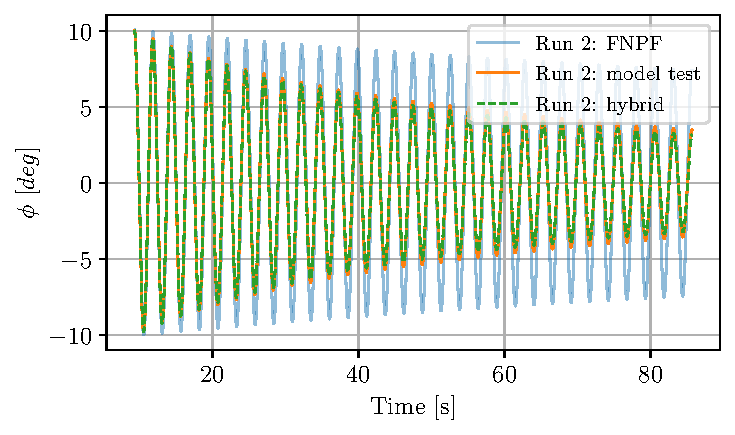
\includegraphics[width = 0.5\textwidth]{figures/hybrid_0_time.pdf}\end{center}
        \vspace{-1cm}
        \caption{Roll decay (0 kn)}
        \label{fig:hybrid_0_time}
    \end{figure}
    
    The roll damping and simulated motions from the hybrid method is similar
to the corresponding model test results for the zero speed case. For the
in speed case the agreement is however even better as seen in the
figures below.

    \begin{figure}[H]
        \begin{center}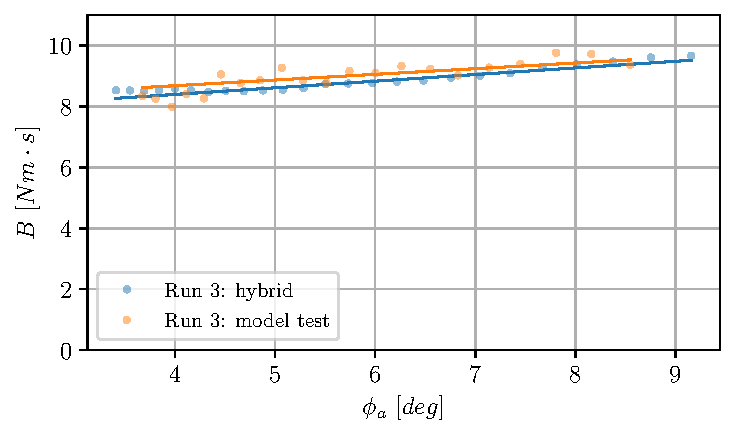
\includegraphics[width = 0.5\textwidth]{figures/hybrid_speed_amplitudes.pdf}\end{center}
        \vspace{-1cm}
        \caption{Total roll damping from hybrid method (15.5 kn)}
        \label{fig:hybrid_speed_amplitudes}
    \end{figure}
    
    \begin{figure}[H]
        \begin{center}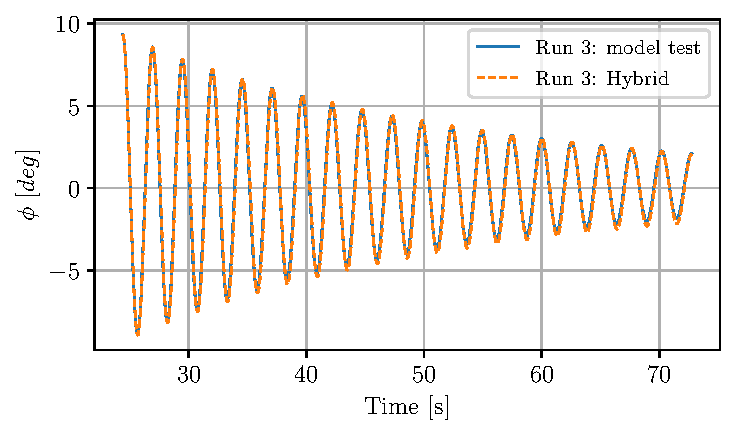
\includegraphics[width = 0.5\textwidth]{figures/hybrid_speed_time.pdf}\end{center}
        \vspace{-1cm}
        \caption{Roll decay (15.5 kn)}
        \label{fig:hybrid_speed_time}
    \end{figure}
    
    The coefficients obtained from model tests, FNPF and hybrid method are
summarized in model scale units in the table below. The equivalent
linearized damping for 5 degrees roll angle amplitude $B_{e5}$ has
also been added to this table. It can be seen that the hybrid method
overpredicts the damping at 0 knots and underpredicts the damping for
the higher speed for this amplitude.
 
            
    
    
\begin{table}[H]
\scriptsize
\center
\caption{Roll damping coefficients for model scale KVLCC2}
\label{tab:results}
\begin{tabular}{llllll}
\toprule\addlinespace
$F_n$ & method & $B_1$ & $B_2$ & $B_3$ & $B_{e5}$\\ 
\midrule$[-]$ &  & $[Nm \cdot s]$ & $[Nm \cdot s^2]$ & $[Nm \cdot s^3]$ & $[Nm \cdot s]$\\ 
0.0 & model test & 2.9604 & -6.5205 & 43.7754 & 3.2864\\ 
0.0 & model test & 2.8797 & -5.8742 & 41.5037 & 3.2447\\ 
0.0 & hybrid & 1.3711 & 13.4769 & 0.0 & 3.828\\ 
0.1423 & model test & 7.5233 & 7.0281 & 0.3898 & 8.8214\\ 
0.1423 & hybrid & 7.5216 & 6.0148 & 0.0 & 8.6095\\ 

\bottomrule
\end{tabular}
\end{table}

    

    